\subsection{Tune measurements}

In the combiner ring the beam does a maximum of 4 turns. 
This makes the situation fundamentally different from a storage ring or 
synchrotron where particles make millions of turns so avoiding the integer or 
half integer resonances are not of the same importance. 
However, tune measurements can give detailed information about the optics and 
possible errors in the machine or in the model.

For the tune measurement the machine was set up for multi turn by shifting 
the timing of the extraction kicker to a later point in time. 
In order to measure the tune the beam was injected 
off the closed orbit into the combiner ring. 
The focusing strength of a quadrupole was changed to observe 
if the changes could be predicted by the model. 
The ideal situation would have been to change quadrupole by 
quadrupole and measure the change in tune.
However, in order to get an accurate tune measurement 
we can only tolerate small beam losses and 
this limits the amount of different settings that could be used.


To measure the tune the following steps have been done. 
They are described in detail in the forthcoming sections.
\begin{enumerate}
\item
Set up the combiner ring so the beam is circulating for at least 60 turns 
without losses.
\item
Acquisition of the signals from the BPMs with different settings of the magnets.
\item
Calculate the beam position for every BPM and every turn.
\item
Determine the average position over several pulses.
\item
Compensate for the charging-up effect.
\item
Fit each signal with a sinusoidal curve.
\item
If the fit is good enough, save the value and put it in the histogram with 
the other BPMs from the same measurement.
\item
Compare the values to the model.
\end{enumerate}


 
Figure \ref{fig:raw_BPM} shows typical traces from a BPM directly read out 
from the control system. In the top the current trace is displayed, 
in the middle the horizontal position and in the bottom the vertical position. 
Every dip marks one turn in the combiner ring. 
At first sight it seems like there were losses along the ring 
since the current is decreasing. 
However, by comparing the offset in the beginning and in the end of the trace, 
it is clear that the offset also has changed. 
Taking this into account we can see that there are only small losses 
in the first turns and then the beam is circulating without any observable losses.

 
The change in the offset is more significant for the BPIs than for the BPMs. 
An example of a signal from a BPI is presented in figure \ref{fig:raw_BPI}. 
In this case it is also possible to see how the position seems to be drifting. 
This phenomena has been known for a long time for this type of devices and 
since it is only observed for the BPIs enables us to conclude that 
it is not a real drift.  
 

In the BPIs the charging up effect is much larger and 
in this case it also affects the position measurement, 
which is shown in figure \ref{fig:raw_BPI}. 
Since we can not see this effect on the BPMs we conclude that 
the drift is not real and the effect can be filtered out. 
This is done by fitting the function with a second degree polynomial and 
then subtracking this from the signal. 
We also took several pulses with the same settings and 
then took the average pulses and calculated the error bar for the position. 
 
 
An example of a fit over the position is presented in figure \ref{fig:fitOfPosition}. 
Normally the turns 4-12 was used to fit. 
An attempt to fit the first turns (1-4) and see if there was a difference 
in tune in the beginning and the end was made. 
It was found that this neither could be ruled out or 
validated because of too big uncertainty in the results, 
stemming from the few turns. 
The reason only the 12 first turns could be used was to the strong dechoherence 
of the oscillation. The oscillation is damped to the closed orbit for the ring. 
Since the beam normally only does 4 turns in the combiner ring 
the closed orbit is not well-determined. 
The closed orbit is interesting to perform different types of measurements to improve 
the understanding of the optics \cite{Minty_Zimmermann_Book}.
\begin{figure}[!h]
\centering
%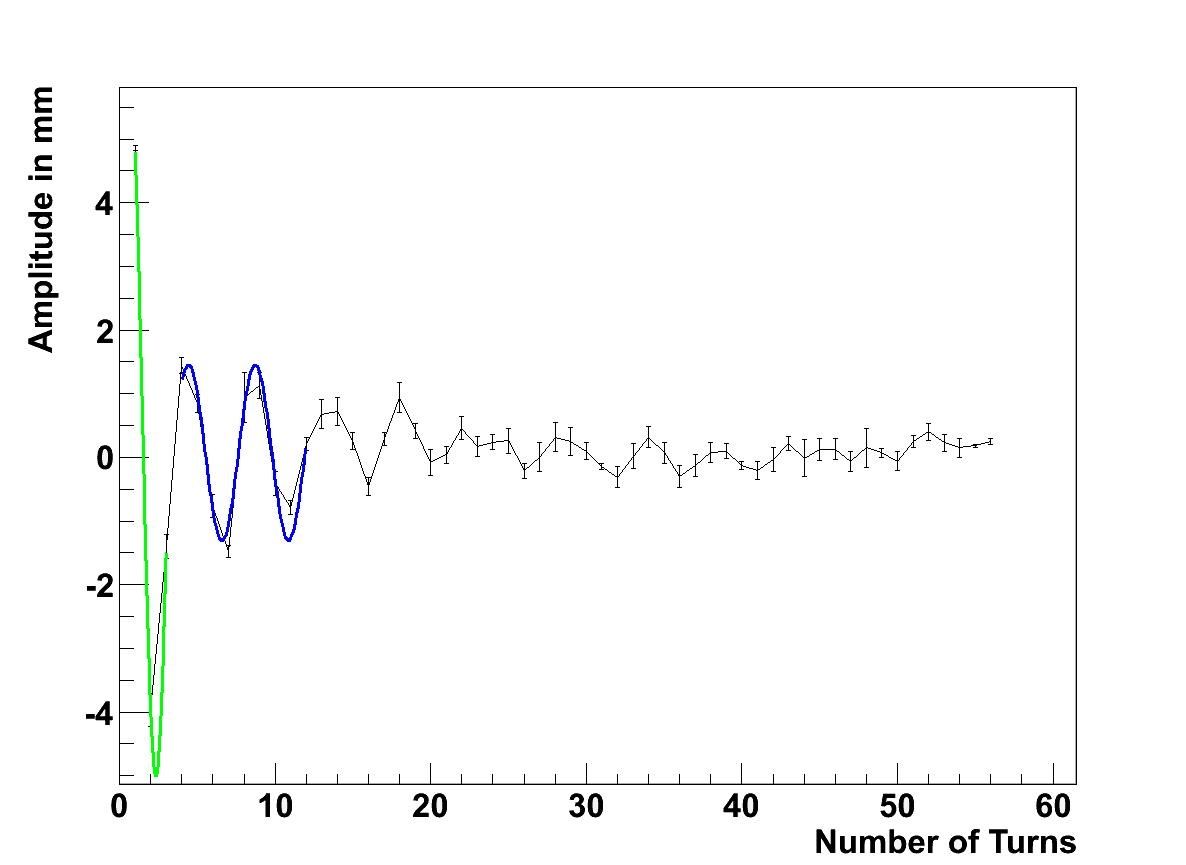
\includegraphics[scale=0.26,natwidth=1186,natheight=865]{fit_BPM8.png}
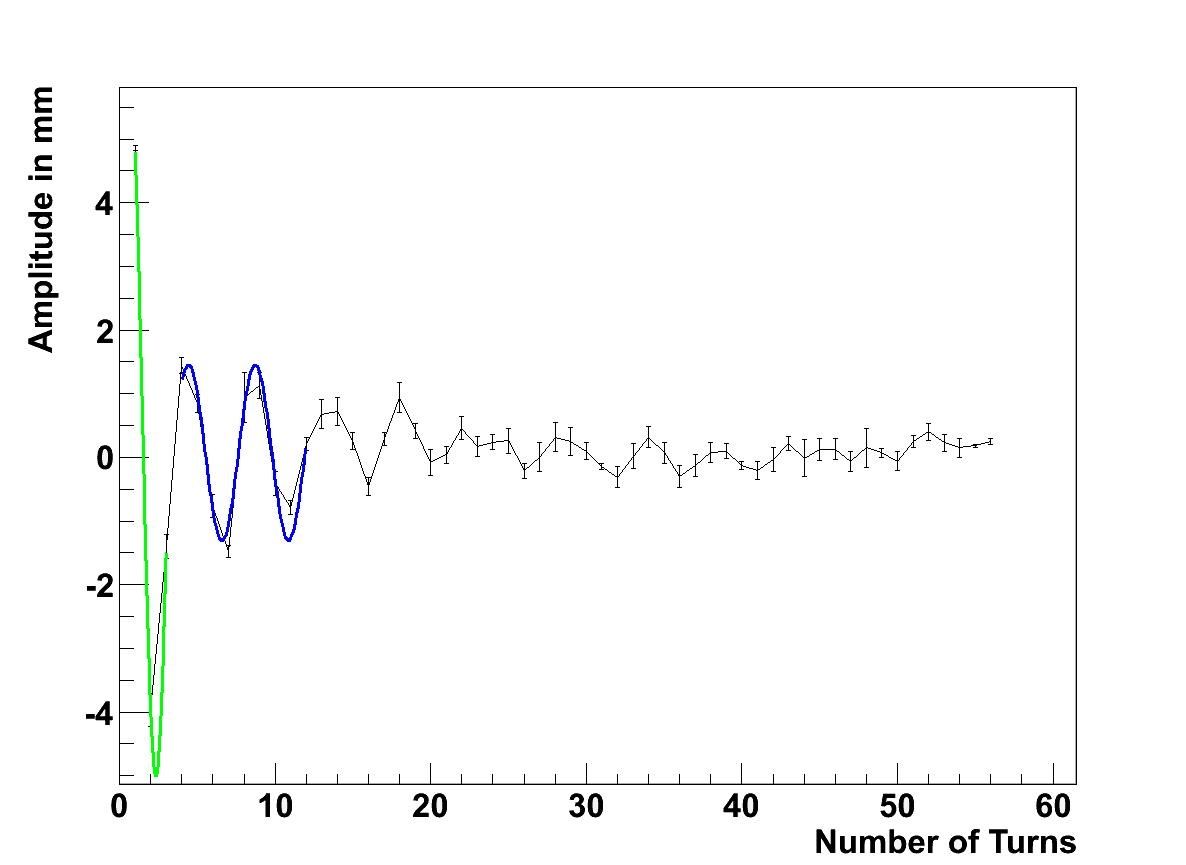
\includegraphics[scale=0.26]{fit_BPM8.png}
\caption{A sinusoidal fit over the position for different turns. \label{fig:fitOfPosition}}
\end{figure}
All fits were checked manually and if seen to fit the signal they were accepted and
placed as a count in a histogram. 
The histogram was then fitted with a Gaussian function and the mean and 
the $\sigma$ were saved for each measurement.
The fact that the tune or period of a sine is 
independent of amplitude of the oscillation makes the tune measurement 
independent of absolute calibration errors in the BPMs.
 
The information we have from each BPM is the position for each turn. 
Since we only have one sampling per turn the maximum tune we can detect is 0.5. 
In the the case of a tune of 0.75 or 0.25, they will look the same, 
due to the aliasing. This can easily be seen from the Nyquist criteria 
which states that we can only see frequencies half the sampling frequency \cite{wiki:nyqvist}. 
In order to determine if we are above or below 0.5, 
we have to change the value of a quadrupole. 
Depending on if the quadrupole is focusing or 
defocusing in that plane and if the tune goes up or down it is possible to 
determine if the tune is above or below 0.5.  

All measurements that were made are summarized in Table~\ref{tab:tuneMeasureTime}. 
The number in the table corresponds to the number on the x-axis in 
Figure~\ref{fig:tuneModelVsMeasureHorizontal} and \ref{fig:tuneModelVsMeasureVertical}
\begin{table}[ht]
\centering
\begin{tabular}{| l | c | c |}
\hline
\textbf{number} & \textbf{time} & \textbf{change} \\ \hline
1 & 09:36:55 & 1\% down \\
2 & 09:34:30 & ref \\
3 & 10:01:31 & 0.5\% down \\
4 & 10:04:45 & 0.6\% down   \\
5 & 10:08:37 & 1.5\% down  \\
6 & 10:16:00 & 0.5\% down  CR.IQFF0510 up 1.5\% \\
7 & 10:27:20 & 0.5\% down  CR.IQFF0510 up 1.7\% \\
8 & 10:30:20 & 0.5\% down  CR.IQFF0510 down 6\% \\
9 & 10:35:00  & 0.5\% down  CR.IQDF0540 down 25\% \\
10 & 10:37:52 &  0.5\% down \\
11 & 10:43:48 &  0.5\% down  CR.IQDF0540 up 5\% \\
12 & 10:48:02 &  0.5\% down  CR.IQDH0340 down 11\% \\
13 & 10:50:05 &  0.5\% down  CR.IQDH0340 up 5\% \\
14 & 10:54:53 &  0.5\% down  quick test with sextupoles \\
\hline
\end{tabular}
\caption[Time and numbering of the tune measurement.]
{The column to the left corresponds to the x-label in 
figure \ref{fig:tuneModelVsMeasureHorizontal} and \ref{fig:tuneModelVsMeasureVertical}. 
The middle column is the time when the measurement was taken and 
the column to the right shows the change in the machine.  \label{tab:tuneMeasureTime}}
\end{table}
\begin{figure}[!h]
\centering
%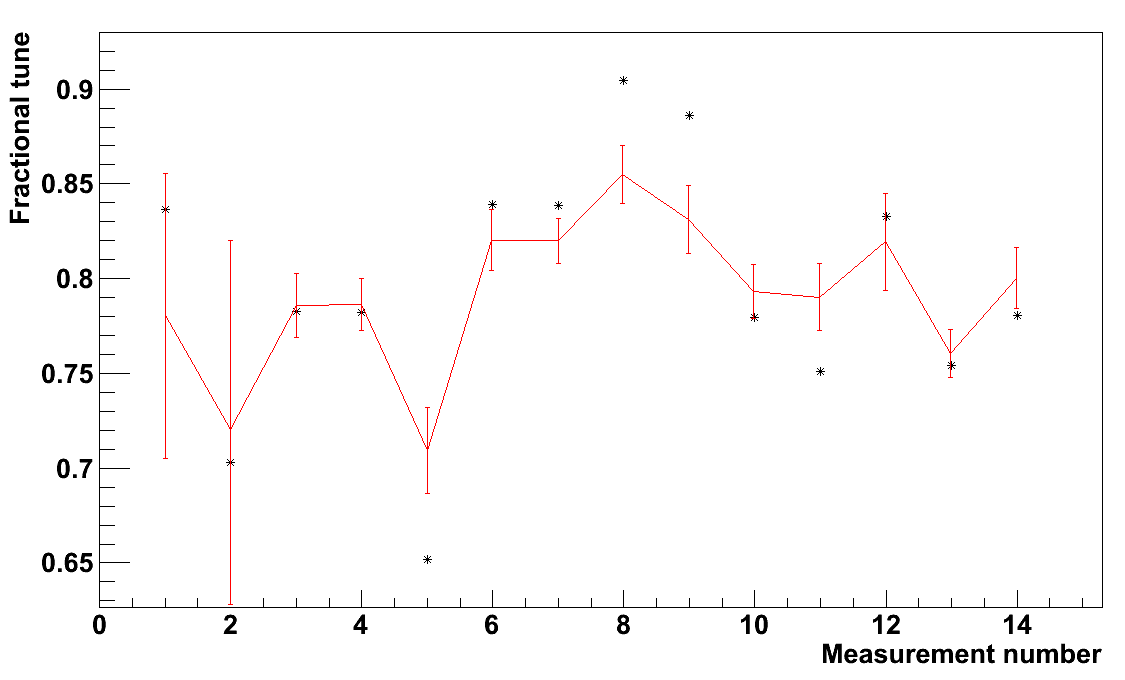
\includegraphics[scale=0.30,natwidth=1253,natheight=719]{horizontal_tuneVsModel.png}
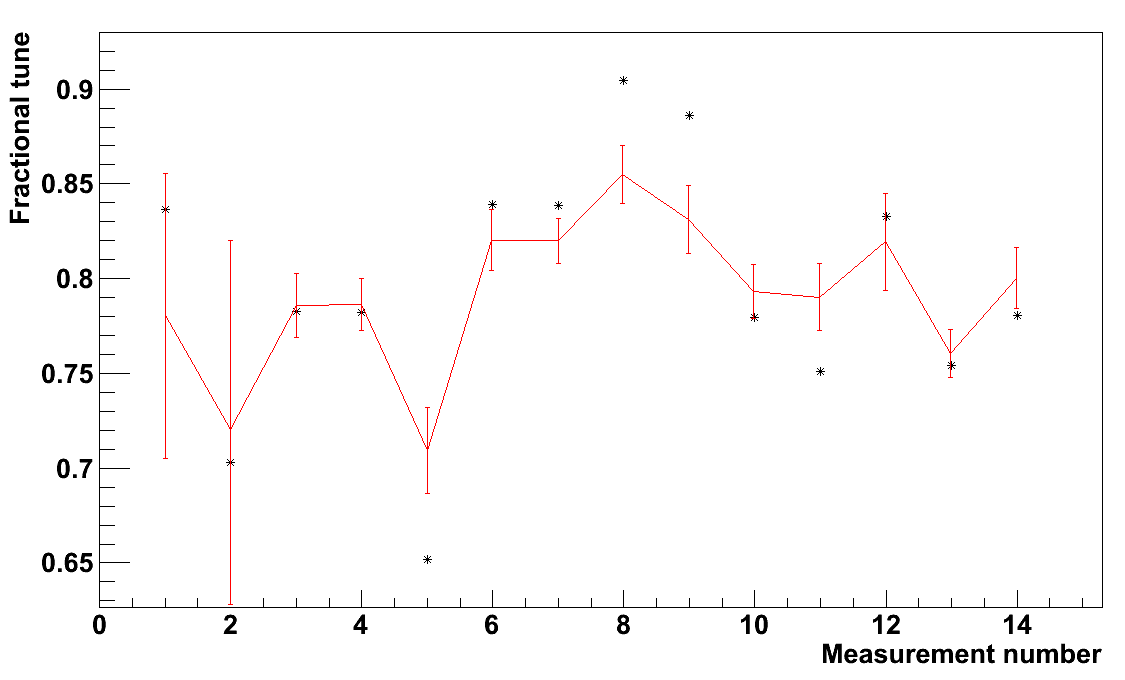
\includegraphics[scale=0.30]{horizontal_tuneVsModel.png}
\caption[Comparison between the tune from the model and the measurement in the horizontal plane]
{Comparison between the model, marked as *, 
and the measurement represented with the red error bars in the horizontal plane. 
\label{fig:tuneModelVsMeasureHorizontal}}
\end{figure}
 
The horizontal tunes for the different measurements series are presented in 
Figure~\ref{fig:tuneModelVsMeasureHorizontal}. 
The model's predictions are in most cases within the error bars 
but for some of the values they are slightly outside. 
Recalling that the error bars are only 1 $\sigma$ we expect 
3 out of 10 points to be outside the error bar, 
thus it is not possible to conclude that there is any error in the model. 
Nevertheless, it seems like the model slightly overestimates 
the change in tune when varying the focusing of a quadrupole.
 
\begin{figure}[!h]
\centering
%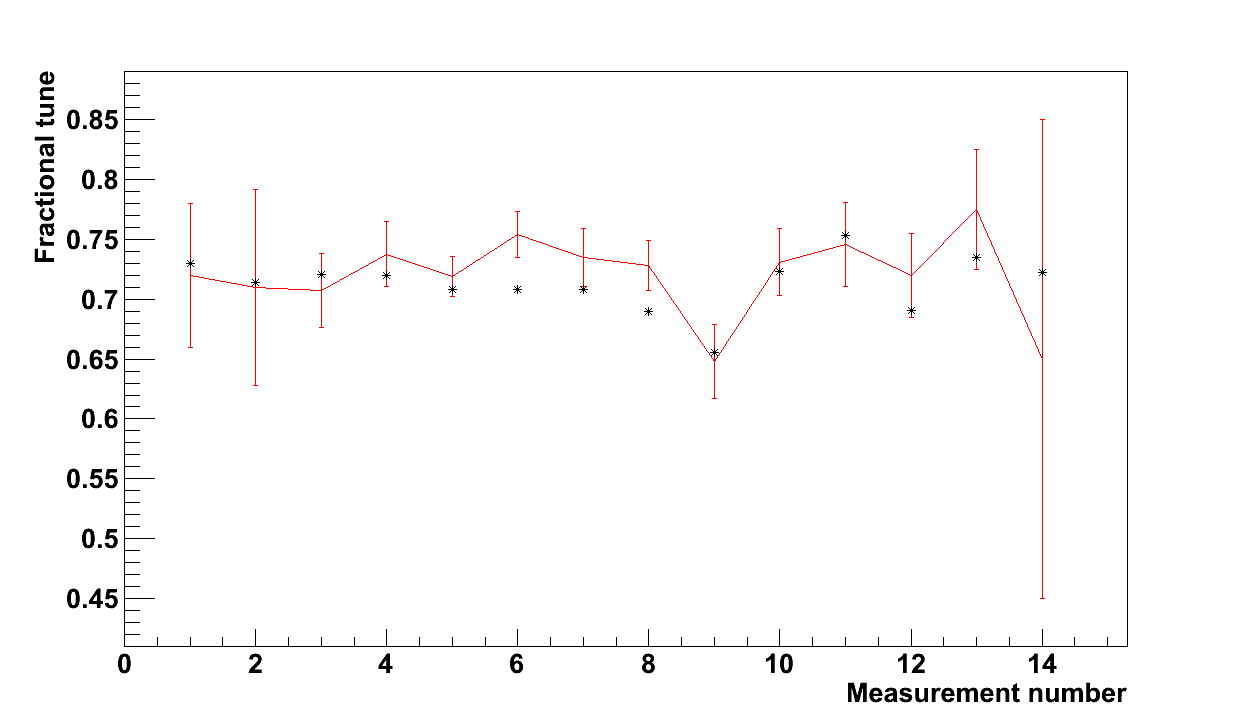
\includegraphics[scale=0.26,natwidth=1253,natheight=719]{vertical_tuneVsModel.png}
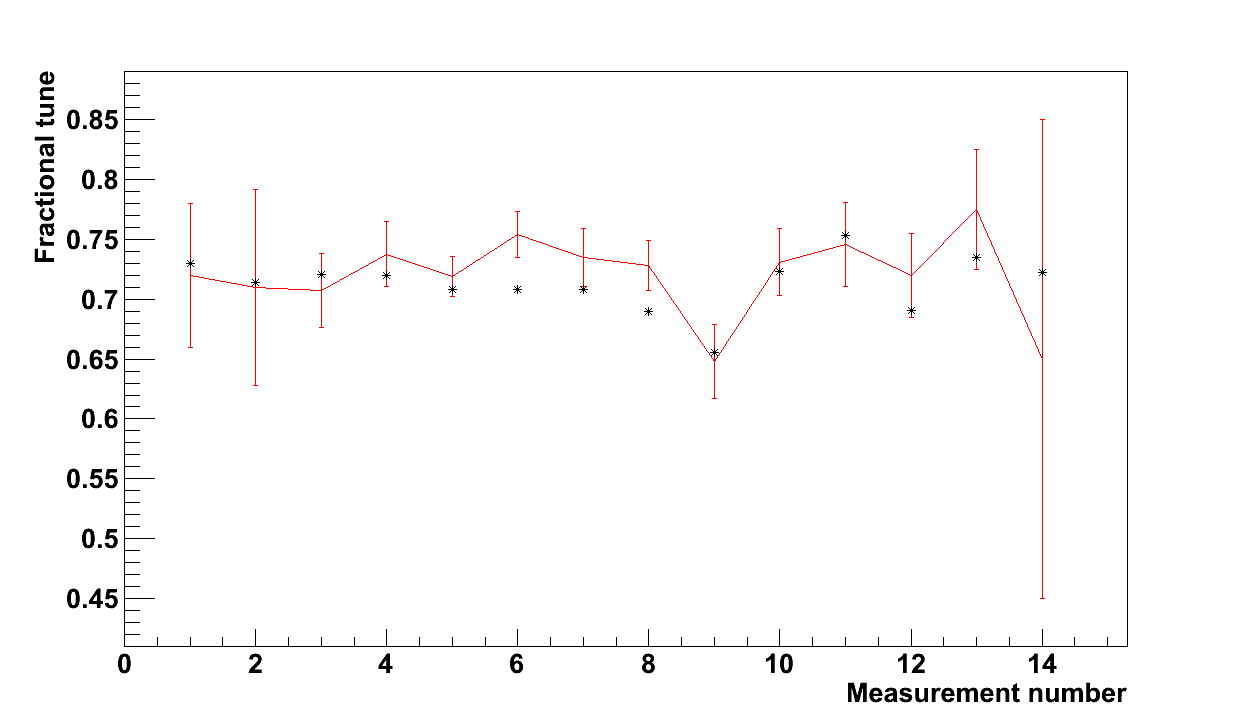
\includegraphics[scale=0.26]{vertical_tuneVsModel.png}
\caption[Comparison between the tune from the model and the measurement in the vertical plane]
{Comparison between the model, marked as *, and the measurement represented with 
the red error bars in the vertical plane \label{fig:tuneModelVsMeasureVertical}}
\end{figure}
In the case of the vertical tune, shown in figure \ref{fig:tuneModelVsMeasureVertical}. 
In this case three points are outside the error bar, which is close to the prediction. 
The fact that one of them is 2 $\sigma$ away is expected if we have 14 points.


The fit also provides information about the phase of each measurement. 
In this case the tune for the fit was fixed to a value obtained in the previous section 
while the tune phase were allowed to vary. 
The phase is aliased but by forcing the fit to be between $0 - \pi$ 
it is possible to compare the phases between different pickups. 
The difference in phase between two successive pickups were added together 
to get the overall phase advance. 
Figure \ref{fig:phaseAdvHorizontal} shows the phase advance for 
the horizontal plane while figure \ref{fig:phaseAdvVertical} shows it 
for the vertical plane. The error bar is 1 $\sigma$ and 
is calculated using the fitting environment in ROOT which takes the error bar into account
when calculating the uncertainty in each parameter.
 
\begin{figure}[!h]
\centering
%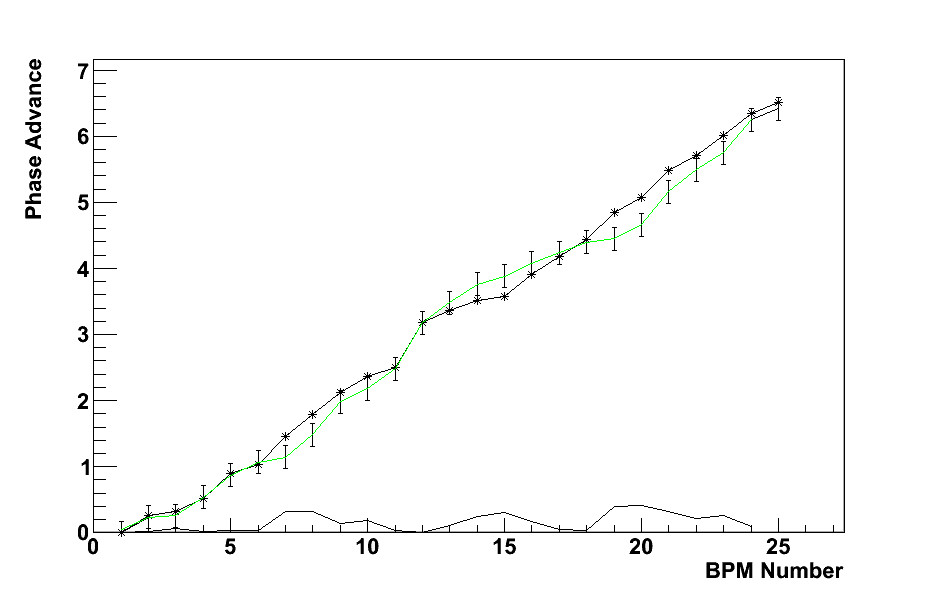
\includegraphics[scale=0.60,natwidth=932,natheight=589]{phaseAdvHorizontal.png}
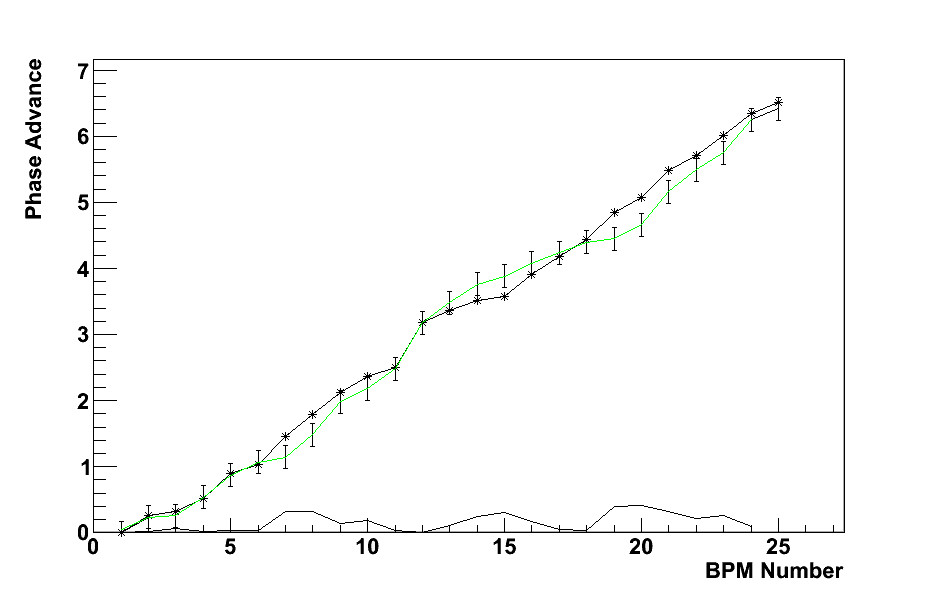
\includegraphics[scale=0.60]{phaseAdvHorizontal.png}
\caption[Phase advance in the horizontal plane]
{Comparison between the model, marked as *, 
and the measurement represented with the green error bars in the horizontal plane. 
The black line shows the absolute difference between the measurement 
and the model. \label{fig:phaseAdvHorizontal}}
\end{figure}
 
\begin{figure}[!h]
\centering
%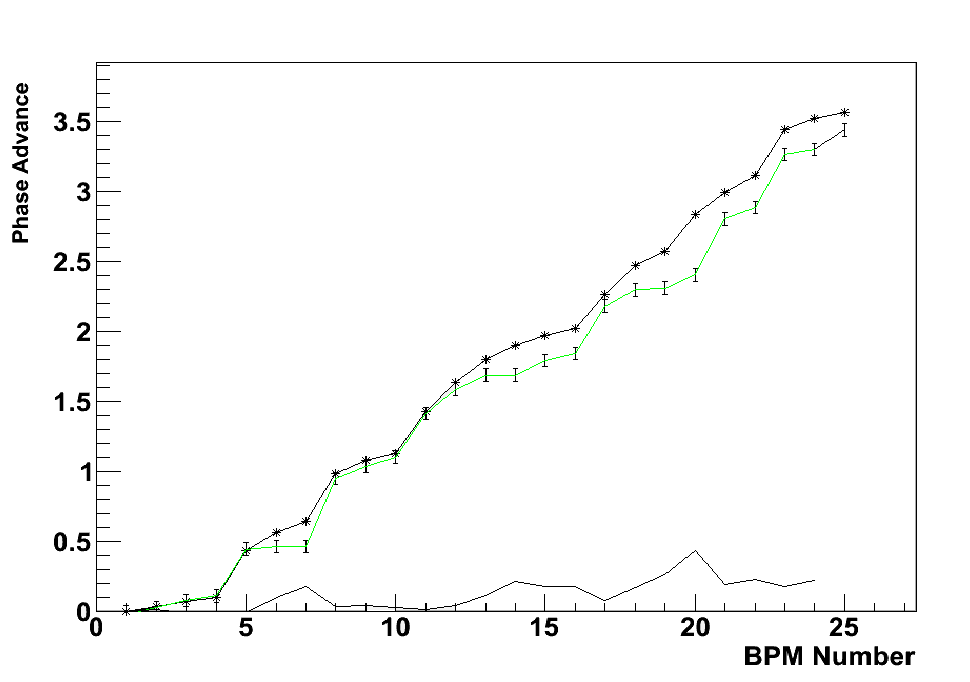
\includegraphics[scale=0.60,natwidth=970,natheight=682]{phaseAdvVertical.png}
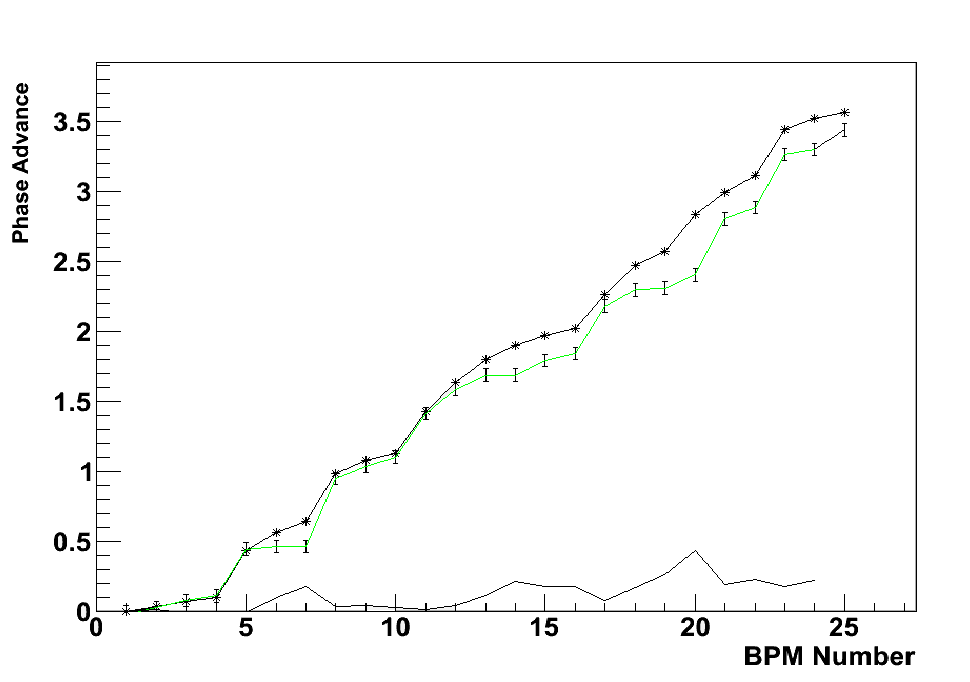
\includegraphics[scale=0.60]{phaseAdvVertical.png}
\caption[Phase advance in the vertical plane]{Comparison between the model, 
marked as *, and the measurement represented with the green error bars 
in the vertical plane. 
The black line shows the absolute difference between the measurement and 
the model.\label{fig:phaseAdvVertical}}
\end{figure}
 
The result is overall in agreement with the model. 
Although, the precision needed to establish if there is a discrepancy 
between the measurement and the model between two consecutive pickups was not achieved. 
However, it provides the additional information that we are close to the design tune. 
With a new optics which corrects for the natural chromaticity more turns will be available
for analysis and increase the precision of the measurements.
 
In order to make more precise measurements it is important 
to be able to have more turns before the oscillation particles dechoere. 
The dechohrence was found to be be mainly due to chromaticity. 
There are sextupoles installed in CTF3 but the achromatic optics is not yet commissioned.
The settings of the sextupoles were found empirically. 
The best result obtained for the vertical oscillation is shown in 
Figure~\ref{fig:tune:sextopole_vertical}. 
This shows that it is possible to use sextupoles to alleviate the effect. 
The fact that we were unable to find a setting to reduce 
the horizontal chromaticity is because the orbit is worse in that plan. 
However, the use of sextupoles introduces extra complexity, 
since the focusing is dependent on the beam position inside the sextupole, 
resulting in a change in tune. 
This effect can be controlled by making sure that the beam passes through the centre of 
the sextupole, if necessary, with the help of correctors \cite{Minty_Zimmermann_Book}. 
The result is in line with a simulation done by Pierre-Louis Pernet \cite{pierre:tune}.    
 
\begin{figure}[!h]
\centering
%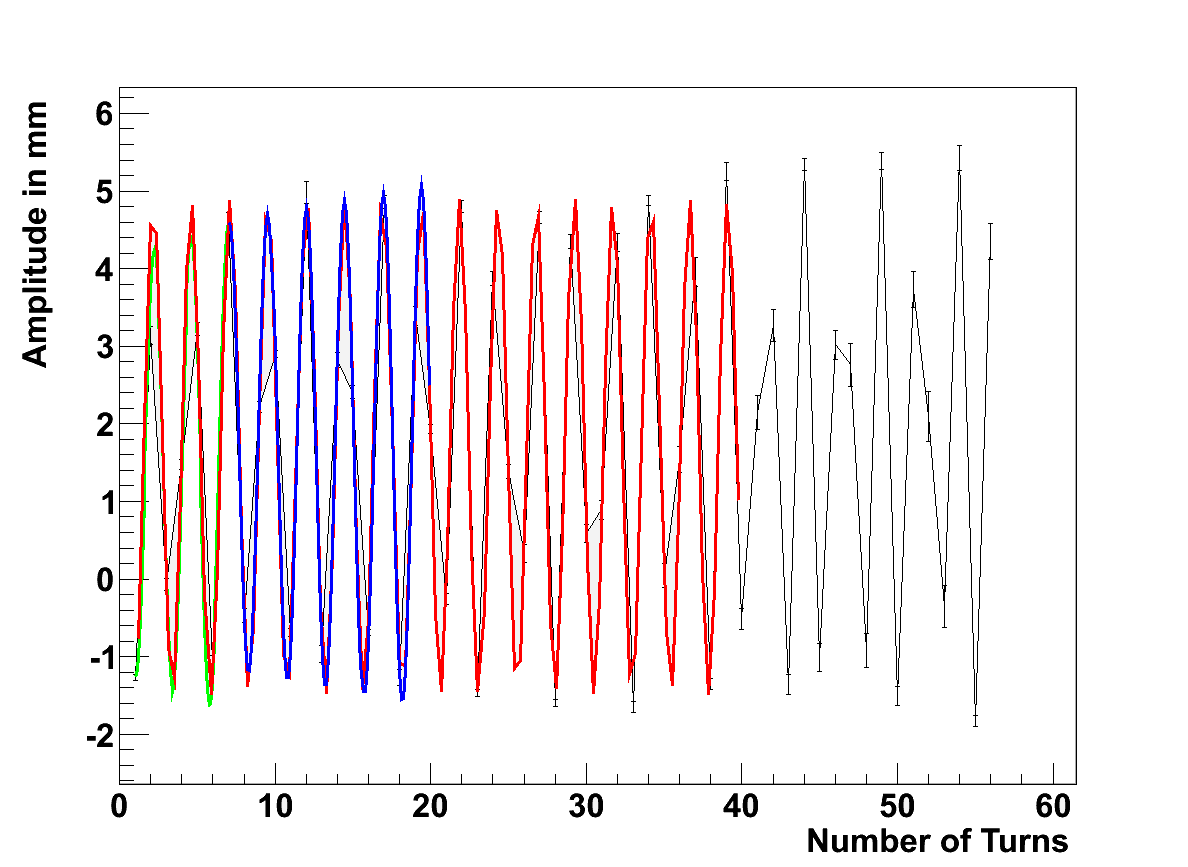
\includegraphics[scale=0.45,natwidth=1188,natheight=867]{sextopole_vertical.png}
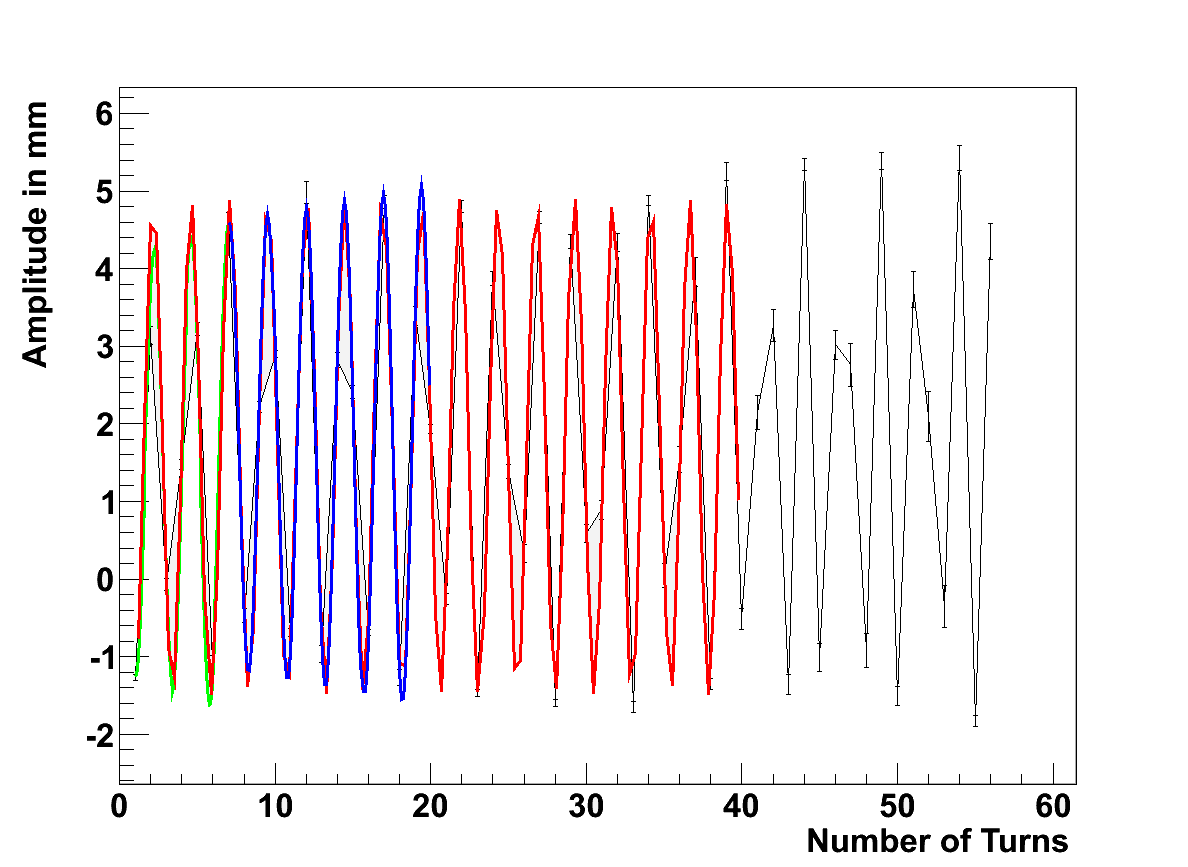
\includegraphics[scale=0.45]{sextopole_vertical.png}
\caption{Vertical oscillation with sextupoles switched on.  \label{fig:tune:sextopole_vertical}}
\end{figure}
 

The overall agreement between the tune measurements and 
the model indicates that there are no major errors in the model. 
In order to reach higher accuracy it is necessary to implement 
the achromatic optics to reduce the chromaticity.
 
